% Created by tikzDevice version 0.12.6 on 2024-03-10 21:16:08
% !TEX encoding = UTF-8 Unicode
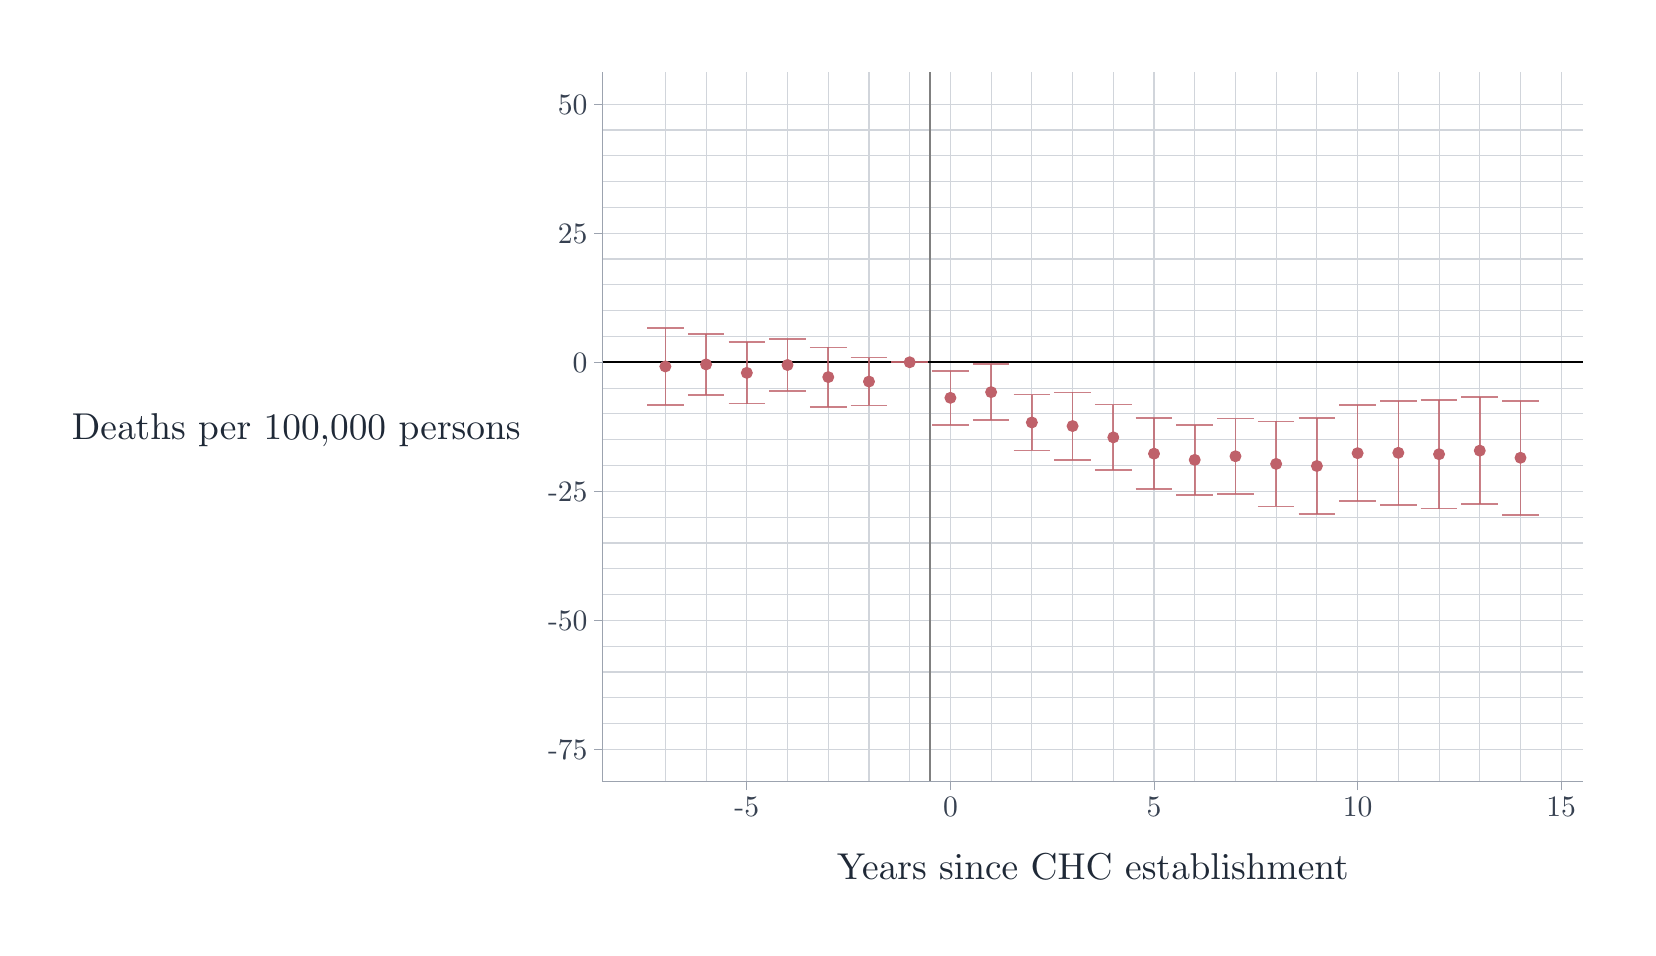
\begin{tikzpicture}[x=1pt,y=1pt]
\definecolor{fillColor}{RGB}{255,255,255}
\path[use as bounding box,fill=fillColor] (0,0) rectangle (578.16,325.21);
\begin{scope}
\path[clip] (  0.00,  0.00) rectangle (578.16,325.21);
\definecolor{drawColor}{RGB}{255,255,255}

\path[draw=drawColor,line width= 0.6pt,line join=round,line cap=round,fill=fillColor] (  0.00,  0.00) rectangle (578.16,325.21);
\end{scope}
\begin{scope}
\path[clip] (207.70, 52.74) rectangle (562.16,309.21);
\definecolor{drawColor}{RGB}{255,255,255}
\definecolor{fillColor}{RGB}{255,255,255}

\path[draw=drawColor,line width= 0.6pt,line join=round,line cap=round,fill=fillColor] (207.70, 52.74) rectangle (562.16,309.22);
\definecolor{drawColor}{RGB}{209,213,219}

\path[draw=drawColor,line width= 0.4pt,line join=round] (207.70, 73.73) --
	(562.16, 73.73);

\path[draw=drawColor,line width= 0.4pt,line join=round] (207.70, 83.06) --
	(562.16, 83.06);

\path[draw=drawColor,line width= 0.4pt,line join=round] (207.70, 92.38) --
	(562.16, 92.38);

\path[draw=drawColor,line width= 0.4pt,line join=round] (207.70,101.71) --
	(562.16,101.71);

\path[draw=drawColor,line width= 0.4pt,line join=round] (207.70,120.36) --
	(562.16,120.36);

\path[draw=drawColor,line width= 0.4pt,line join=round] (207.70,129.69) --
	(562.16,129.69);

\path[draw=drawColor,line width= 0.4pt,line join=round] (207.70,139.01) --
	(562.16,139.01);

\path[draw=drawColor,line width= 0.4pt,line join=round] (207.70,148.34) --
	(562.16,148.34);

\path[draw=drawColor,line width= 0.4pt,line join=round] (207.70,166.99) --
	(562.16,166.99);

\path[draw=drawColor,line width= 0.4pt,line join=round] (207.70,176.32) --
	(562.16,176.32);

\path[draw=drawColor,line width= 0.4pt,line join=round] (207.70,185.64) --
	(562.16,185.64);

\path[draw=drawColor,line width= 0.4pt,line join=round] (207.70,194.97) --
	(562.16,194.97);

\path[draw=drawColor,line width= 0.4pt,line join=round] (207.70,213.62) --
	(562.16,213.62);

\path[draw=drawColor,line width= 0.4pt,line join=round] (207.70,222.95) --
	(562.16,222.95);

\path[draw=drawColor,line width= 0.4pt,line join=round] (207.70,232.27) --
	(562.16,232.27);

\path[draw=drawColor,line width= 0.4pt,line join=round] (207.70,241.60) --
	(562.16,241.60);

\path[draw=drawColor,line width= 0.4pt,line join=round] (207.70,260.25) --
	(562.16,260.25);

\path[draw=drawColor,line width= 0.4pt,line join=round] (207.70,269.58) --
	(562.16,269.58);

\path[draw=drawColor,line width= 0.4pt,line join=round] (207.70,278.90) --
	(562.16,278.90);

\path[draw=drawColor,line width= 0.4pt,line join=round] (207.70,288.23) --
	(562.16,288.23);

\path[draw=drawColor,line width= 0.4pt,line join=round] (230.43, 52.74) --
	(230.43,309.21);

\path[draw=drawColor,line width= 0.4pt,line join=round] (245.14, 52.74) --
	(245.14,309.21);

\path[draw=drawColor,line width= 0.4pt,line join=round] (274.57, 52.74) --
	(274.57,309.21);

\path[draw=drawColor,line width= 0.4pt,line join=round] (289.29, 52.74) --
	(289.29,309.21);

\path[draw=drawColor,line width= 0.4pt,line join=round] (304.00, 52.74) --
	(304.00,309.21);

\path[draw=drawColor,line width= 0.4pt,line join=round] (318.71, 52.74) --
	(318.71,309.21);

\path[draw=drawColor,line width= 0.4pt,line join=round] (348.14, 52.74) --
	(348.14,309.21);

\path[draw=drawColor,line width= 0.4pt,line join=round] (362.86, 52.74) --
	(362.86,309.21);

\path[draw=drawColor,line width= 0.4pt,line join=round] (377.57, 52.74) --
	(377.57,309.21);

\path[draw=drawColor,line width= 0.4pt,line join=round] (392.29, 52.74) --
	(392.29,309.21);

\path[draw=drawColor,line width= 0.4pt,line join=round] (421.71, 52.74) --
	(421.71,309.21);

\path[draw=drawColor,line width= 0.4pt,line join=round] (436.43, 52.74) --
	(436.43,309.21);

\path[draw=drawColor,line width= 0.4pt,line join=round] (451.14, 52.74) --
	(451.14,309.21);

\path[draw=drawColor,line width= 0.4pt,line join=round] (465.86, 52.74) --
	(465.86,309.21);

\path[draw=drawColor,line width= 0.4pt,line join=round] (495.28, 52.74) --
	(495.28,309.21);

\path[draw=drawColor,line width= 0.4pt,line join=round] (510.00, 52.74) --
	(510.00,309.21);

\path[draw=drawColor,line width= 0.4pt,line join=round] (524.71, 52.74) --
	(524.71,309.21);

\path[draw=drawColor,line width= 0.4pt,line join=round] (539.43, 52.74) --
	(539.43,309.21);

\path[draw=drawColor,line width= 0.4pt,line join=round] (207.70, 64.40) --
	(562.16, 64.40);

\path[draw=drawColor,line width= 0.4pt,line join=round] (207.70,111.03) --
	(562.16,111.03);

\path[draw=drawColor,line width= 0.4pt,line join=round] (207.70,157.66) --
	(562.16,157.66);

\path[draw=drawColor,line width= 0.4pt,line join=round] (207.70,204.30) --
	(562.16,204.30);

\path[draw=drawColor,line width= 0.4pt,line join=round] (207.70,250.93) --
	(562.16,250.93);

\path[draw=drawColor,line width= 0.4pt,line join=round] (207.70,297.56) --
	(562.16,297.56);

\path[draw=drawColor,line width= 0.4pt,line join=round] (259.86, 52.74) --
	(259.86,309.21);

\path[draw=drawColor,line width= 0.4pt,line join=round] (333.43, 52.74) --
	(333.43,309.21);

\path[draw=drawColor,line width= 0.4pt,line join=round] (407.00, 52.74) --
	(407.00,309.21);

\path[draw=drawColor,line width= 0.4pt,line join=round] (480.57, 52.74) --
	(480.57,309.21);

\path[draw=drawColor,line width= 0.4pt,line join=round] (554.14, 52.74) --
	(554.14,309.21);
\definecolor{drawColor}{gray}{0.50}

\path[draw=drawColor,line width= 0.6pt,line join=round] (326.07, 52.74) -- (326.07,309.21);
\definecolor{drawColor}{RGB}{0,0,0}

\path[draw=drawColor,line width= 0.6pt,line join=round] (207.70,204.30) -- (562.16,204.30);
\definecolor{drawColor}{RGB}{191,97,106}
\definecolor{fillColor}{RGB}{191,97,106}

\path[draw=drawColor,line width= 0.4pt,line join=round,line cap=round,fill=fillColor] (230.43,202.79) circle (  1.96);

\path[draw=drawColor,line width= 0.4pt,line join=round,line cap=round,fill=fillColor] (245.14,203.53) circle (  1.96);

\path[draw=drawColor,line width= 0.4pt,line join=round,line cap=round,fill=fillColor] (259.86,200.47) circle (  1.96);

\path[draw=drawColor,line width= 0.4pt,line join=round,line cap=round,fill=fillColor] (274.57,203.31) circle (  1.96);

\path[draw=drawColor,line width= 0.4pt,line join=round,line cap=round,fill=fillColor] (289.29,198.94) circle (  1.96);

\path[draw=drawColor,line width= 0.4pt,line join=round,line cap=round,fill=fillColor] (304.00,197.33) circle (  1.96);

\path[draw=drawColor,line width= 0.4pt,line join=round,line cap=round,fill=fillColor] (333.43,191.45) circle (  1.96);

\path[draw=drawColor,line width= 0.4pt,line join=round,line cap=round,fill=fillColor] (348.14,193.51) circle (  1.96);

\path[draw=drawColor,line width= 0.4pt,line join=round,line cap=round,fill=fillColor] (362.86,182.55) circle (  1.96);

\path[draw=drawColor,line width= 0.4pt,line join=round,line cap=round,fill=fillColor] (377.57,181.25) circle (  1.96);

\path[draw=drawColor,line width= 0.4pt,line join=round,line cap=round,fill=fillColor] (392.29,177.16) circle (  1.96);

\path[draw=drawColor,line width= 0.4pt,line join=round,line cap=round,fill=fillColor] (407.00,171.28) circle (  1.96);

\path[draw=drawColor,line width= 0.4pt,line join=round,line cap=round,fill=fillColor] (421.71,169.03) circle (  1.96);

\path[draw=drawColor,line width= 0.4pt,line join=round,line cap=round,fill=fillColor] (436.43,170.34) circle (  1.96);

\path[draw=drawColor,line width= 0.4pt,line join=round,line cap=round,fill=fillColor] (451.14,167.57) circle (  1.96);

\path[draw=drawColor,line width= 0.4pt,line join=round,line cap=round,fill=fillColor] (465.86,166.81) circle (  1.96);

\path[draw=drawColor,line width= 0.4pt,line join=round,line cap=round,fill=fillColor] (480.57,171.45) circle (  1.96);

\path[draw=drawColor,line width= 0.4pt,line join=round,line cap=round,fill=fillColor] (495.28,171.58) circle (  1.96);

\path[draw=drawColor,line width= 0.4pt,line join=round,line cap=round,fill=fillColor] (510.00,171.08) circle (  1.96);

\path[draw=drawColor,line width= 0.4pt,line join=round,line cap=round,fill=fillColor] (524.71,172.37) circle (  1.96);

\path[draw=drawColor,line width= 0.4pt,line join=round,line cap=round,fill=fillColor] (539.43,169.79) circle (  1.96);

\path[draw=drawColor,line width= 0.4pt,line join=round,line cap=round,fill=fillColor] (318.71,204.30) circle (  1.96);
\definecolor{drawColor}{RGB}{191,97,106}

\path[draw=drawColor,draw opacity=0.80,line width= 0.6pt,line join=round] (223.81,216.62) --
	(237.05,216.62);

\path[draw=drawColor,draw opacity=0.80,line width= 0.6pt,line join=round] (230.43,216.62) --
	(230.43,188.95);

\path[draw=drawColor,draw opacity=0.80,line width= 0.6pt,line join=round] (223.81,188.95) --
	(237.05,188.95);

\path[draw=drawColor,draw opacity=0.80,line width= 0.6pt,line join=round] (238.52,214.61) --
	(251.77,214.61);

\path[draw=drawColor,draw opacity=0.80,line width= 0.6pt,line join=round] (245.14,214.61) --
	(245.14,192.44);

\path[draw=drawColor,draw opacity=0.80,line width= 0.6pt,line join=round] (238.52,192.44) --
	(251.77,192.44);

\path[draw=drawColor,draw opacity=0.80,line width= 0.6pt,line join=round] (253.24,211.59) --
	(266.48,211.59);

\path[draw=drawColor,draw opacity=0.80,line width= 0.6pt,line join=round] (259.86,211.59) --
	(259.86,189.36);

\path[draw=drawColor,draw opacity=0.80,line width= 0.6pt,line join=round] (253.24,189.36) --
	(266.48,189.36);

\path[draw=drawColor,draw opacity=0.80,line width= 0.6pt,line join=round] (267.95,212.67) --
	(281.19,212.67);

\path[draw=drawColor,draw opacity=0.80,line width= 0.6pt,line join=round] (274.57,212.67) --
	(274.57,193.95);

\path[draw=drawColor,draw opacity=0.80,line width= 0.6pt,line join=round] (267.95,193.95) --
	(281.19,193.95);

\path[draw=drawColor,draw opacity=0.80,line width= 0.6pt,line join=round] (282.67,209.67) --
	(295.91,209.67);

\path[draw=drawColor,draw opacity=0.80,line width= 0.6pt,line join=round] (289.29,209.67) --
	(289.29,188.20);

\path[draw=drawColor,draw opacity=0.80,line width= 0.6pt,line join=round] (282.67,188.20) --
	(295.91,188.20);

\path[draw=drawColor,draw opacity=0.80,line width= 0.6pt,line join=round] (297.38,205.97) --
	(310.62,205.97);

\path[draw=drawColor,draw opacity=0.80,line width= 0.6pt,line join=round] (304.00,205.97) --
	(304.00,188.68);

\path[draw=drawColor,draw opacity=0.80,line width= 0.6pt,line join=round] (297.38,188.68) --
	(310.62,188.68);

\path[draw=drawColor,draw opacity=0.80,line width= 0.6pt,line join=round] (326.81,201.18) --
	(340.05,201.18);

\path[draw=drawColor,draw opacity=0.80,line width= 0.6pt,line join=round] (333.43,201.18) --
	(333.43,181.71);

\path[draw=drawColor,draw opacity=0.80,line width= 0.6pt,line join=round] (326.81,181.71) --
	(340.05,181.71);

\path[draw=drawColor,draw opacity=0.80,line width= 0.6pt,line join=round] (341.52,203.58) --
	(354.76,203.58);

\path[draw=drawColor,draw opacity=0.80,line width= 0.6pt,line join=round] (348.14,203.58) --
	(348.14,183.45);

\path[draw=drawColor,draw opacity=0.80,line width= 0.6pt,line join=round] (341.52,183.45) --
	(354.76,183.45);

\path[draw=drawColor,draw opacity=0.80,line width= 0.6pt,line join=round] (356.24,192.63) --
	(369.48,192.63);

\path[draw=drawColor,draw opacity=0.80,line width= 0.6pt,line join=round] (362.86,192.63) --
	(362.86,172.47);

\path[draw=drawColor,draw opacity=0.80,line width= 0.6pt,line join=round] (356.24,172.47) --
	(369.48,172.47);

\path[draw=drawColor,draw opacity=0.80,line width= 0.6pt,line join=round] (370.95,193.41) --
	(384.19,193.41);

\path[draw=drawColor,draw opacity=0.80,line width= 0.6pt,line join=round] (377.57,193.41) --
	(377.57,169.09);

\path[draw=drawColor,draw opacity=0.80,line width= 0.6pt,line join=round] (370.95,169.09) --
	(384.19,169.09);

\path[draw=drawColor,draw opacity=0.80,line width= 0.6pt,line join=round] (385.66,189.04) --
	(398.91,189.04);

\path[draw=drawColor,draw opacity=0.80,line width= 0.6pt,line join=round] (392.29,189.04) --
	(392.29,165.27);

\path[draw=drawColor,draw opacity=0.80,line width= 0.6pt,line join=round] (385.66,165.27) --
	(398.91,165.27);

\path[draw=drawColor,draw opacity=0.80,line width= 0.6pt,line join=round] (400.38,184.11) --
	(413.62,184.11);

\path[draw=drawColor,draw opacity=0.80,line width= 0.6pt,line join=round] (407.00,184.11) --
	(407.00,158.45);

\path[draw=drawColor,draw opacity=0.80,line width= 0.6pt,line join=round] (400.38,158.45) --
	(413.62,158.45);

\path[draw=drawColor,draw opacity=0.80,line width= 0.6pt,line join=round] (415.09,181.60) --
	(428.34,181.60);

\path[draw=drawColor,draw opacity=0.80,line width= 0.6pt,line join=round] (421.71,181.60) --
	(421.71,156.45);

\path[draw=drawColor,draw opacity=0.80,line width= 0.6pt,line join=round] (415.09,156.45) --
	(428.34,156.45);

\path[draw=drawColor,draw opacity=0.80,line width= 0.6pt,line join=round] (429.81,183.94) --
	(443.05,183.94);

\path[draw=drawColor,draw opacity=0.80,line width= 0.6pt,line join=round] (436.43,183.94) --
	(436.43,156.74);

\path[draw=drawColor,draw opacity=0.80,line width= 0.6pt,line join=round] (429.81,156.74) --
	(443.05,156.74);

\path[draw=drawColor,draw opacity=0.80,line width= 0.6pt,line join=round] (444.52,182.91) --
	(457.76,182.91);

\path[draw=drawColor,draw opacity=0.80,line width= 0.6pt,line join=round] (451.14,182.91) --
	(451.14,152.22);

\path[draw=drawColor,draw opacity=0.80,line width= 0.6pt,line join=round] (444.52,152.22) --
	(457.76,152.22);

\path[draw=drawColor,draw opacity=0.80,line width= 0.6pt,line join=round] (459.23,184.10) --
	(472.48,184.10);

\path[draw=drawColor,draw opacity=0.80,line width= 0.6pt,line join=round] (465.86,184.10) --
	(465.86,149.53);

\path[draw=drawColor,draw opacity=0.80,line width= 0.6pt,line join=round] (459.23,149.53) --
	(472.48,149.53);

\path[draw=drawColor,draw opacity=0.80,line width= 0.6pt,line join=round] (473.95,188.81) --
	(487.19,188.81);

\path[draw=drawColor,draw opacity=0.80,line width= 0.6pt,line join=round] (480.57,188.81) --
	(480.57,154.08);

\path[draw=drawColor,draw opacity=0.80,line width= 0.6pt,line join=round] (473.95,154.08) --
	(487.19,154.08);

\path[draw=drawColor,draw opacity=0.80,line width= 0.6pt,line join=round] (488.66,190.41) --
	(501.91,190.41);

\path[draw=drawColor,draw opacity=0.80,line width= 0.6pt,line join=round] (495.28,190.41) --
	(495.28,152.76);

\path[draw=drawColor,draw opacity=0.80,line width= 0.6pt,line join=round] (488.66,152.76) --
	(501.91,152.76);

\path[draw=drawColor,draw opacity=0.80,line width= 0.6pt,line join=round] (503.38,190.71) --
	(516.62,190.71);

\path[draw=drawColor,draw opacity=0.80,line width= 0.6pt,line join=round] (510.00,190.71) --
	(510.00,151.45);

\path[draw=drawColor,draw opacity=0.80,line width= 0.6pt,line join=round] (503.38,151.45) --
	(516.62,151.45);

\path[draw=drawColor,draw opacity=0.80,line width= 0.6pt,line join=round] (518.09,191.66) --
	(531.33,191.66);

\path[draw=drawColor,draw opacity=0.80,line width= 0.6pt,line join=round] (524.71,191.66) --
	(524.71,153.08);

\path[draw=drawColor,draw opacity=0.80,line width= 0.6pt,line join=round] (518.09,153.08) --
	(531.33,153.08);

\path[draw=drawColor,draw opacity=0.80,line width= 0.6pt,line join=round] (532.81,190.42) --
	(546.05,190.42);

\path[draw=drawColor,draw opacity=0.80,line width= 0.6pt,line join=round] (539.43,190.42) --
	(539.43,149.15);

\path[draw=drawColor,draw opacity=0.80,line width= 0.6pt,line join=round] (532.81,149.15) --
	(546.05,149.15);

\path[draw=drawColor,draw opacity=0.80,line width= 0.6pt,line join=round] (312.09,204.30) --
	(325.34,204.30);

\path[draw=drawColor,draw opacity=0.80,line width= 0.6pt,line join=round] (318.71,204.30) --
	(318.71,204.30);

\path[draw=drawColor,draw opacity=0.80,line width= 0.6pt,line join=round] (312.09,204.30) --
	(325.34,204.30);
\end{scope}
\begin{scope}
\path[clip] (  0.00,  0.00) rectangle (578.16,325.21);
\definecolor{drawColor}{RGB}{156,163,175}

\path[draw=drawColor,line width= 0.3pt,line join=round] (207.70, 52.74) --
	(207.70,309.21);
\end{scope}
\begin{scope}
\path[clip] (  0.00,  0.00) rectangle (578.16,325.21);
\definecolor{drawColor}{RGB}{55,65,81}

\node[text=drawColor,anchor=base east,inner sep=0pt, outer sep=0pt, scale=  1.07] at (202.30, 60.73) {-75};

\node[text=drawColor,anchor=base east,inner sep=0pt, outer sep=0pt, scale=  1.07] at (202.30,107.36) {-50};

\node[text=drawColor,anchor=base east,inner sep=0pt, outer sep=0pt, scale=  1.07] at (202.30,153.99) {-25};

\node[text=drawColor,anchor=base east,inner sep=0pt, outer sep=0pt, scale=  1.07] at (202.30,200.62) {0};

\node[text=drawColor,anchor=base east,inner sep=0pt, outer sep=0pt, scale=  1.07] at (202.30,247.25) {25};

\node[text=drawColor,anchor=base east,inner sep=0pt, outer sep=0pt, scale=  1.07] at (202.30,293.88) {50};
\end{scope}
\begin{scope}
\path[clip] (  0.00,  0.00) rectangle (578.16,325.21);
\definecolor{drawColor}{RGB}{156,163,175}

\path[draw=drawColor,line width= 0.3pt,line join=round] (204.70, 64.40) --
	(207.70, 64.40);

\path[draw=drawColor,line width= 0.3pt,line join=round] (204.70,111.03) --
	(207.70,111.03);

\path[draw=drawColor,line width= 0.3pt,line join=round] (204.70,157.66) --
	(207.70,157.66);

\path[draw=drawColor,line width= 0.3pt,line join=round] (204.70,204.30) --
	(207.70,204.30);

\path[draw=drawColor,line width= 0.3pt,line join=round] (204.70,250.93) --
	(207.70,250.93);

\path[draw=drawColor,line width= 0.3pt,line join=round] (204.70,297.56) --
	(207.70,297.56);
\end{scope}
\begin{scope}
\path[clip] (  0.00,  0.00) rectangle (578.16,325.21);
\definecolor{drawColor}{RGB}{156,163,175}

\path[draw=drawColor,line width= 0.3pt,line join=round] (207.70, 52.74) --
	(562.16, 52.74);
\end{scope}
\begin{scope}
\path[clip] (  0.00,  0.00) rectangle (578.16,325.21);
\definecolor{drawColor}{RGB}{156,163,175}

\path[draw=drawColor,line width= 0.3pt,line join=round] (259.86, 49.74) --
	(259.86, 52.74);

\path[draw=drawColor,line width= 0.3pt,line join=round] (333.43, 49.74) --
	(333.43, 52.74);

\path[draw=drawColor,line width= 0.3pt,line join=round] (407.00, 49.74) --
	(407.00, 52.74);

\path[draw=drawColor,line width= 0.3pt,line join=round] (480.57, 49.74) --
	(480.57, 52.74);

\path[draw=drawColor,line width= 0.3pt,line join=round] (554.14, 49.74) --
	(554.14, 52.74);
\end{scope}
\begin{scope}
\path[clip] (  0.00,  0.00) rectangle (578.16,325.21);
\definecolor{drawColor}{RGB}{55,65,81}

\node[text=drawColor,anchor=base,inner sep=0pt, outer sep=0pt, scale=  1.07] at (259.86, 40.00) {-5};

\node[text=drawColor,anchor=base,inner sep=0pt, outer sep=0pt, scale=  1.07] at (333.43, 40.00) {0};

\node[text=drawColor,anchor=base,inner sep=0pt, outer sep=0pt, scale=  1.07] at (407.00, 40.00) {5};

\node[text=drawColor,anchor=base,inner sep=0pt, outer sep=0pt, scale=  1.07] at (480.57, 40.00) {10};

\node[text=drawColor,anchor=base,inner sep=0pt, outer sep=0pt, scale=  1.07] at (554.14, 40.00) {15};
\end{scope}
\begin{scope}
\path[clip] (  0.00,  0.00) rectangle (578.16,325.21);
\definecolor{drawColor}{RGB}{31,41,55}

\node[text=drawColor,anchor=base,inner sep=0pt, outer sep=0pt, scale=  1.35] at (384.93, 17.31) {Years since CHC establishment};
\end{scope}
\begin{scope}
\path[clip] (  0.00,  0.00) rectangle (578.16,325.21);
\definecolor{drawColor}{RGB}{31,41,55}

\node[text=drawColor,anchor=base,inner sep=0pt, outer sep=0pt, scale=  1.35] at ( 97.04,176.33) {Deaths per 100,000 persons};
\end{scope}
\end{tikzpicture}
